\section{Vorbetrachtung}
\label{sec:relatedwork}

Als erstes gilt es, gegenwärtige Technologien zu evaluieren, um eine solide Grundlage für eine verteilte Dateiverwaltung für die Schul-Cloud zu erstellen. Wie in der Einleitung erwähnt wurde, soll kein neuartiges Dateiverwaltungskonzept geschaffen werden. Vielmehr soll auf bestehenden Systemen und Technologien aufgebaut werden und deren Vorteile genutzt werden. Somit schließt sich eine Beobachtung an, inwieweit Dateiablagen auf Basis von Cloud-Storage Provider bereits im Unterricht genutzt werden. Danach werden im Vorfeld formulierte Anforderungen aufgegriffen und analysiert. Hierzu diente der Technischen Bericht der Schul-Cloud \cite{paper:technischerbericht} als Grundlage, welcher in Zusammenarbeit des Hasso-Plattner-Instut mit dem Mint-EC enstand. Für eine abschließende Vorbetrachtung eignet sich eine Betrachtung bereits bestehender Cloud-Storage Anbieter, welche sich in der Praxis bewährt haben und weiträumigen Einsatz finden.

\subsection{Nutzung von Cloud-Storage Provider im Unterricht}

Die Verwaltung von eigenen und geteilten Dateien wird mit der zunehmenden Digitalisierung des Unterrichts immer wichtiger. Wo es früher reichte, seine Unterrichtsmaterialen in einem Schulhefter zu legen, will man Arbeitsblätter und Wissenstexte heute überall und immer verfügbar haben. Um einen Eindruck in diese Problematik zu bekommen, wurde eine Umfrage zum Thema 'Dateiorganisation in der Schule' \cite{survey:umfragedateiorganisation} erstellt und an ehemaligen und aktuellen Schülern und Lehrern geschickt. Insgesamt namen \textbf{\textit{65}} \todo{Anpassen} Teilnehmer  an dieser Umfrage teil. Gefragt wurde unter anderem nach der Rolle des Teilnehmers (Schüler oder Lehrer) gefragt [Frage 1]. Dabei sollten ehemalige Schüler und Lehrer vergangene Erfahrungen in die Beantwortung der Frage einfließen lassen. Dann wurde danach gefragt, ob der Befragte webbasierte Anwendungen zur Verwaltung der Dateien im Schulalltag benutzt hat [Frage 2]. Anschließend wurde die Befragung geteilt. Wenn die Frage 2 mit 'Nein' beantwortet wurde, wurde nach Gründen für das Nichtbenutzen gefragt [Frage 3]. Wurde Frage 2 mit 'Ja' beantwortet, wurde nach Vorteilen der Nutzung gefragt [Frage 4], sowie nach Beispielen, welche Dienste genutzt wurden [Frage 5]. 

\cite{survey:umfragedateiorganisationergebnisse}

\todo[inline]{Todo: Umfrage auswerten}

\subsection{Anforderungen an die Schul-Cloud}

\begin{center}
	
	\begin{figure}[H]
		\begin{center}
			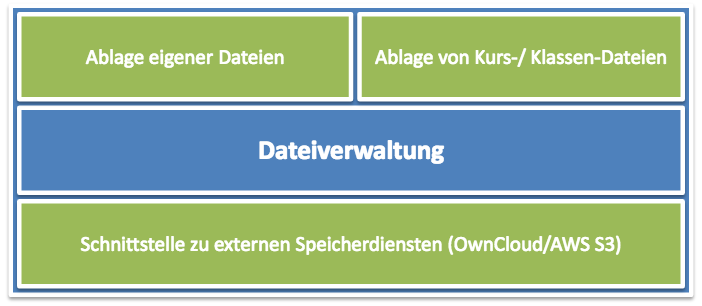
\includegraphics[width=0.8\linewidth]{images/AnforderungenDateiverwaltung}
			\caption[Caption for relatedWork]{Grundanforderungen an die Dateiverwaltung der Schul-Cloud\footnotemark}
			\label{fig:devices}
		\end{center}
	\end{figure}
	\footnotetext{Martin Hense (Mint-EC - https://www.mint-ec.de/)}
\end{center}


\subsection{Bestehende Cloud-Storage Provider}

\todo[inline]{Todo: AWS S3 OwnCloud}

\clearpage
